
\documentclass[fleqn,10pt]{wlscirep}
\usepackage[utf8]{inputenc}
\usepackage[T1]{fontenc}
\usepackage{tabularx}
\usepackage{array}
\usepackage{booktabs}
\usepackage{url}
\usepackage{float}
\usepackage{amsmath}
\usepackage{lineno}
\newcolumntype{Y}{>{\raggedright\arraybackslash}X}
\newcolumntype{L}[1]{>{\raggedright\arraybackslash}p{#1}}
\Urlmuskip=0mu plus 1mu
\emergencystretch=3em

\title{Validation controlled imbalance aware learning for fine grained IoT intrusion detection}

\author[1,2]{Junjie Zhang}
\author[1,*]{Siyu Wang}
\affil[1]{Shanghai Academy of Global Governance \& Area Studies, Shanghai International Studies University, Shanghai 201620, China; Junjie Zhang: junjiezhang2024@shisu.edu.cn; junjiezhang1720@163.com}
\affil[2]{School of Economics and Finance, Shanghai International Studies University, Shanghai 201620, China}
\affil[*]{Correspondence: Siyu Wang, wangsiyu\_real@126.com}

\begin{abstract}
Fine grained Internet of Things intrusion detection remains difficult because high aggregate accuracy can hide weak recall for rare attack labels. We evaluate validation controlled imbalance handling with a probability ensemble whose mixing weight is selected only on an internal validation split. On the CICIoT2023 public subsample, the selected ensemble increased Macro-F1 from 0.8612 to 0.8828 and minority recall, defined as recall for the lowest support test class, from 0.1910 to 0.5131. IoTID20 repeated holdouts supported a split stable recall pattern: top ten weighted LightGBM improved Macro-F1 by 0.0140 and minority recall by 0.2129 relative to flat LightGBM, but did not support universal ensemble superiority. In N-BaIoT, binary and family tasks were near saturated under a capped leave one device out setting, whereas fine grained attack labels were more device dependent. The results support validation controlled imbalance handling as a reproducible evaluation discipline, rather than a universal claim for one ensemble across datasets.
\end{abstract}

\begin{document}
\raggedbottom
\sloppy
\maketitle
\thispagestyle{empty}

\noindent\textbf{Keywords:} Internet of Things; intrusion detection; class imbalance; rare attack recognition; ensemble learning; external validation

\section*{Introduction}

Internet of Things (IoT) systems are now embedded in homes, healthcare, transportation, manufacturing and smart city infrastructure \cite{alfuqaha2015iot,roman2013iotsecurity,sicari2015iottrust}. Intrusion detection in these environments cannot stop at benign versus malicious separation. Fine grained attack recognition matters because reconnaissance, spoofing, denial of service and malware related events call for different mitigation decisions. High overall accuracy can still leave rare attack categories poorly recognized.

Public intrusion detection datasets have made reproducible IoT and network security evaluation more feasible, including CICIoT2023, IoTID20, N-BaIoT, UNSW-NB15, CICIDS2017, Bot-IoT and Edge-IIoTset \cite{neto2023ciciot,ullah2020iotid20,meidan2018nbaiot,moustafa2015unsw,sharafaldin2018cicids,koroniotis2019botiot,ferrag2022edgeiiot}. These datasets also expose a persistent evaluation problem: aggregate scores can obscure weak recognition of low support labels.

A central difficulty is class imbalance. Modern machine learning models learn dominant IoT traffic patterns efficiently, but majority labels can also dominate loss functions, validation choices and headline performance measures \cite{he2009imbalanced,branco2016imbalanced,krawczyk2016imbalanced}. Accuracy is therefore a weak security metric when rare labels have low recall. Macro-F1, balanced accuracy, macro precision recall area and minority recall give a more direct view of fine grained intrusion detection.

Existing strategies solve only part of the problem. Gradient tree boosting provides a strong tabular learner for this setting \cite{chen2016xgboost}. SMOTE and Borderline-SMOTE increase exposure to underrepresented classes, although synthetic samples can be unreliable when the minority boundary is noisy \cite{chawla2002smote,han2005borderline}. Class weighting increases sensitivity to rare classes, often at the cost of precision or global class balance. Ensembles can combine operating points \cite{galar2012ensembles}, but many intrusion detection studies use fixed weights or select configurations after repeated observation of test performance. Such designs risk optimistic evaluation because the ensemble configuration is influenced directly or indirectly by the test data.

The recent literature is also broad in model family. Traditional machine learning studies still report competitive results with tree models and feature selection because network flow tables are structured and high dimensional. Deep learning studies use convolutional, recurrent, attention and transformer style models to learn richer traffic representations. Other work combines feature selection with large language model based augmentation, focal loss or class sensitive objectives to address imbalance. Edge and lightweight intrusion detection studies add an efficiency constraint because a detector may need to run near constrained devices. These strands are useful, but they answer different questions: some emphasize architecture novelty, some emphasize accuracy, and some emphasize computational cost.

The methodological gap is therefore not simply the absence of another classifier. Recent Scientific Reports studies show that machine learning intrusion detection remains active \cite{alsubaei2025smart,yu2025attack,amine2025improved,ma2025llm,sarwar2025securing,singh2025attentional}, while a supervised intrusion detection review highlights fragmentation across datasets, metrics and evaluation criteria \cite{abushareha2026review}. Several studies report high headline accuracy or detection rate under their own data splits and task definitions. Those results are important field context, but they are not direct substitutes for rare class recall, frozen test evaluation, repeated split uncertainty and device held out validation. Supplementary Table S11 therefore compares recent Scientific Reports and adjacent intrusion detection studies by validation design rather than treating incompatible headline scores as a leaderboard.

This manuscript consequently makes a conservative claim. It does not propose a new deep architecture and it does not claim the highest reported accuracy on the complete original CICIoT2023 corpus. Instead, it asks whether imbalance aware model choices can be fixed by validation data and then evaluated under a controlled evidence chain. The answer matters because a high accuracy detector that misses rare attacks may be less useful than a detector with a slightly lower global score but a better documented rare class operating point.

We address this gap by treating validation control as part of the learning framework. A Borderline-SMOTE LightGBM component and a class weighted XGBoost component are mixed through a probability weight selected on internal validation data only \cite{chen2016xgboost}. Final performance on the CICIoT2023 public subsample is evaluated once on a frozen test split \cite{neto2023ciciot}. IoTID20 \cite{ullah2020iotid20} and N-BaIoT \cite{meidan2018nbaiot} are used as boundary checks for split stability and generalization to unseen devices, not as extra leaderboard claims. Additional public intrusion detection datasets motivate the broader benchmark context \cite{moustafa2015unsw,sharafaldin2018cicids,koroniotis2019botiot,ferrag2022edgeiiot}.

The study makes three contributions. First, it introduces a reusable model selection framework that controls validation for imbalanced multi class security classification. Second, it evaluates the framework with rare class metrics, bootstrap uncertainty, repeated holdouts and capped leave one device out validation. Third, it shows that the transferable finding is imbalance aware validation and weighting rather than a universal claim that one ensemble dominates every dataset. The article next reports the validation evidence, discusses the boundaries of the claim and then provides the full implementation details needed for reproduction.

\section*{Methods}

\subsection*{Study framework}

Three validation roles structure the study (Figure~\ref{fig:design}). The CICIoT2023 public subsample serves as the primary confirmatory benchmark because it provides a large public fine grained IoT attack setting. IoTID20 is an independent check of split stability with repeated stratified holdouts. N-BaIoT is a capped validation problem where each device is removed completely from training and used as an unseen test device.

\begin{figure}[H]
\centering
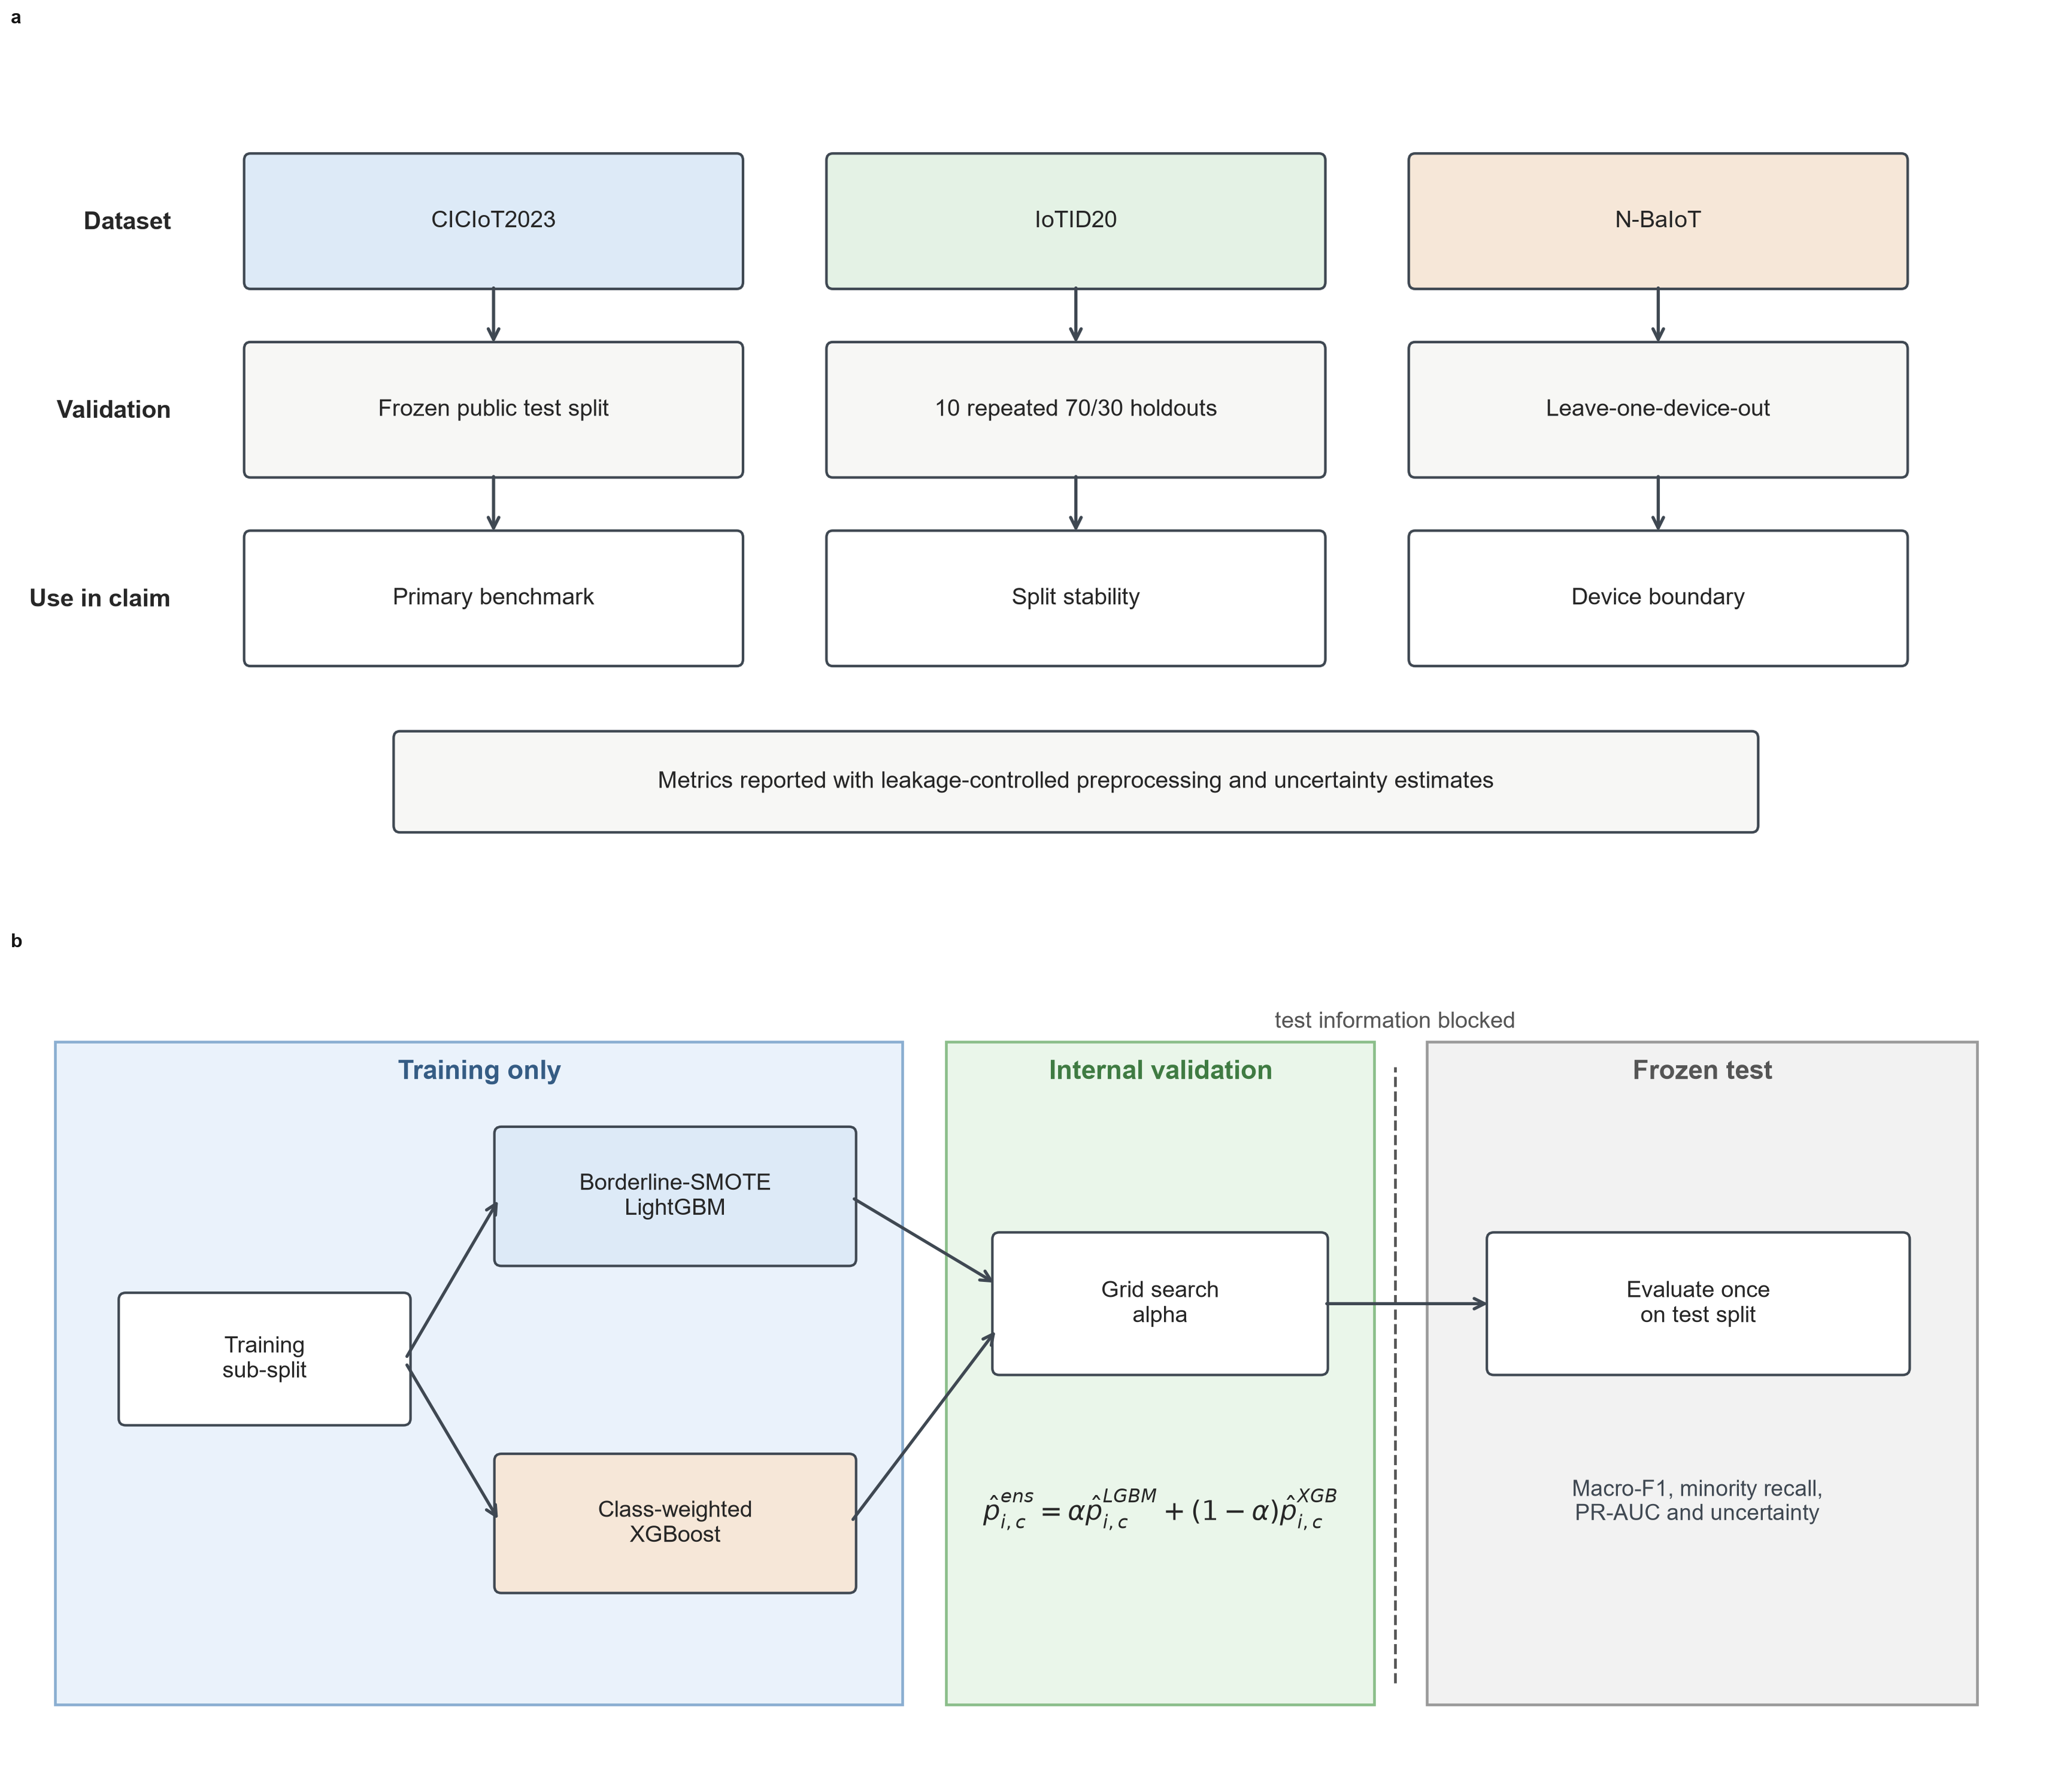
\includegraphics[width=0.98\linewidth]{figures/figure1_study_validation_framework.png}
\caption{\textbf{Study and validation control framework.}}
\label{fig:design}
\end{figure}

\subsection*{Validation-controlled ensemble method}

Probability mixing uses two complementary components (Figure~\ref{fig:design}). Borderline-SMOTE LightGBM supplies the component that preserves Macro-F1. XGBoost with class weights supplies the component that is sensitive to recall. For the CICIoT2023 public subsample, the 1,143,802 row training split was further divided into an 80\% fitting split and a 20\% validation split with stratified sampling and random seed 42. The mixing weight $\alpha$ was selected only on this validation split. For observation $i$ and class $c$, the ensemble probability is

\begin{equation}
\hat{p}_{i,c}^{ens}(\alpha)
=
\alpha \hat{p}_{i,c}^{LGBM}
+
(1-\alpha)\hat{p}_{i,c}^{XGB},
\label{eq:ensemble}
\end{equation}

where $\hat{p}_{i,c}^{LGBM}$ and $\hat{p}_{i,c}^{XGB}$ are component probabilities and $\alpha$ is selected from 0.00 to 1.00 in increments of 0.05. The convex constraint keeps the output on the probability simplex and prevents extrapolation beyond the two fitted components. On the CICIoT2023 public subsample, both Macro-F1 and a composite Macro-F1 plus minority recall objective selected $\alpha=0.50$; the validation curve is reported in Supplementary Figure S2.

Operationally, validation controlled ensemble selection used a fixed six step sequence. First, the CICIoT2023 public subsample training file was divided into fitting and internal validation subsets by stratified sampling. Second, Borderline-SMOTE LightGBM and class weighted XGBoost were fitted only on the fitting subset. Third, candidate values of $\alpha$ from 0.00 to 1.00 were evaluated on the internal validation subset. Fourth, the selected $\alpha$ was frozen before any test set prediction was inspected. Finally, both components were refitted on the full training split and evaluated once on the frozen CICIoT2023 public subsample test split.

\subsection*{Dataset preparation and leakage control}

Only numeric traffic features were used. The CICIoT2023 public subsample contained 47 numeric predictors after label and metadata columns were excluded. Non finite values were replaced with missing values and then imputed as zero for CICIoT2023 public subsample tree models; IoTID20 rows with missing or infinite values were removed before splitting. No categorical feature encoding was applied because categorical labels and identifiers were excluded from the feature matrix unless a variable was explicitly part of the task definition. Label encoders were fitted on training data only. Feature ranking, oversampling and class weight computation were also fitted within the training portion of each split. For the CICIoT2023 public subsample, the predefined test file was not used for feature selection, model choice, threshold tuning or ensemble weight selection.

The IoTID20 repeated experiment used 10 stratified 70/30 holdouts with seeds 42 through 51. Fixed factors included data cleaning, feature space, model hyperparameters, class weighting and the top ten mutual information feature selection procedure. The varying factor was the split seed. The N-BaIoT experiment used a cap of 20,000 rows per source file after non finite rows were removed. Leave one device out folds were then constructed so that each held out device represented an unseen entity rather than a random subset of the same device traffic. Table~\ref{tab:design} summarizes the dataset roles and leakage control rules.

\begin{table}[H]
\centering
\caption{\textbf{Dataset roles and validation design.} Each dataset was assigned a distinct inferential role so that primary performance, repeated split stability and unseen-device generalization are not collapsed into a single overbroad claim.}
\label{tab:design}
\small
\begin{tabularx}{\linewidth}{L{2.15cm} L{2.65cm} L{2.25cm} L{2.55cm} Y}
\toprule
Dataset & Role & Rows used & Target & Leakage-control rule \\
\midrule
CICIoT2023 public subsample & Primary confirmatory benchmark & 1,143,802 train; 285,951 test & 34 fine grained labels & Predefined test split frozen; internal validation only for alpha selection \\
IoTID20 public mirror & Repeated independent holdout replication & 625,783 after cleaning & Nine labels & Ten stratified 70/30 splits; training-only feature ranking; split-level bootstrap \\
N-BaIoT UCI archive & Capped unseen device validation & 1,772,641 after cleaning & Binary, family and attack labels & One complete device held out in each fold \\
\bottomrule
\end{tabularx}
\end{table}

\subsection*{Evaluation metrics}

The primary metric for fine grained classification was Macro-F1. Secondary metrics included accuracy, balanced accuracy, macro precision recall area, weighted F1, minority recall, worst class recall and inference time per 1,000 rows. Precision recall analysis is particularly informative under class imbalance \cite{davis2006pr,saito2015pr}. Minority recall was defined as

\begin{equation}
R_{minority} =
\frac{1}{|\mathcal{C}_{min}|}
\sum_{c \in \mathcal{C}_{min}}
\frac{TP_c}{TP_c + FN_c},
\label{eq:minority}
\end{equation}

where $\mathcal{C}_{min}=\left\{c:n_c=\min_j n_j,\ n_j>0\right\}$ is the set of classes with the lowest positive support in the evaluation split, $n_c$ is the support of class $c$, and $TP_c$ and $FN_c$ are true positives and false negatives for class $c$. In the CICIoT2023 public subsample test split, this set contains Uploading\_Attack only, with 267 test rows. Figure~\ref{fig:ciciot-main} is a separate diagnostic for the four lowest support attack labels and is not the definition of minority recall. For N-BaIoT, Macro-F1 for classes present in the fold was also reported because some held out devices lack attack labels that are present in the training devices.

\subsection*{Statistical analysis}

For the main CICIoT2023 public subsample comparison, paired row bootstrap intervals were computed on the frozen test file using 2,000 resamples \cite{efron1979bootstrap,efron1987bca}. These intervals quantify uncertainty from resampling the fixed test file; they do not estimate uncertainty from alternative CICIoT2023 public subsample train test partitions. That limitation is deliberate because the public subsample test split was kept frozen. Split uncertainty is instead examined in IoTID20. For IoTID20, paired deltas were computed at the split level for each of the 10 repeated holdouts:

\begin{equation}
\Delta M_s = M_{A,s} - M_{B,s}, \qquad s=1,\ldots,S,
\label{eq:splitdelta}
\end{equation}

where $M_{A,s}$ is the metric for the imbalance-aware model, $M_{B,s}$ is the metric for flat LightGBM and $S=10$ for IoTID20. Percentile intervals were estimated from 10,000 bootstrap resamples of the paired split-level deltas:

\begin{equation}
\mathrm{CI}_{1-\gamma} =
\left[
q_{\gamma/2}\left(\Delta M^*\right),
q_{1-\gamma/2}\left(\Delta M^*\right)
\right],
\label{eq:bootstrap}
\end{equation}

where $\Delta M^*$ is the bootstrap distribution of paired performance differences and $q$ denotes the empirical quantile.

As a second check for IoTID20, an exact sign flip test was applied to the 10 paired split level deltas \cite{dietterich1998tests,ernst2004permutation}. The null distribution was generated by all $2^{10}$ possible sign assignments to the paired deltas. This test is reported as a robustness check for direction consistency rather than as a replacement for effect sizes and intervals.

\subsection*{Software and reproducibility}

Analyses were implemented in Python using pandas, scikit learn, imbalanced learn, LightGBM, XGBoost, NumPy, matplotlib, seaborn and SHAP \cite{lundberg2020shap}. Package requirements are pinned in \texttt{requirements.txt}. LightGBM used 220 estimators, learning rate 0.06, 63 leaves and \texttt{random\_state=42}. XGBoost used 220 estimators, maximum depth 7, learning rate 0.08 and the histogram tree method. Borderline-SMOTE used an adaptive \texttt{k\_neighbors} value from 1 to 5 according to the smallest training class; \texttt{m\_neighbors} used the imbalanced learn default. All stochastic splits, model seeds, bootstrap resamples and SHAP sampling steps used fixed random seeds recorded in the executable scripts. Experiments were run on Windows 11 with an AMD Ryzen 9 8945HS processor and 31.3 GB RAM. Runtime and model complexity records are reported in Supplementary Table S7. AI assisted coding and drafting tools were used to help generate scripts, check numerical consistency and improve manuscript wording; the authors reviewed all generated text and verified all numerical claims against result files.

\section*{Results}

\subsection*{CICIoT2023 public subsample validation performance}

To determine whether validation controlled selection improves fine grained intrusion detection under severe class imbalance, the CICIoT2023 public subsample was used as the primary benchmark. Flat LightGBM reached high accuracy but weak minority recall. The ensemble selected on internal validation data raised Macro-F1 from 0.8612 to 0.8828 and minority recall from 0.1910 to 0.5131. Macro PR-AUC also increased from 0.8863 to 0.9219 (Figure~\ref{fig:ciciot-main}).

\begin{figure}[H]
\centering
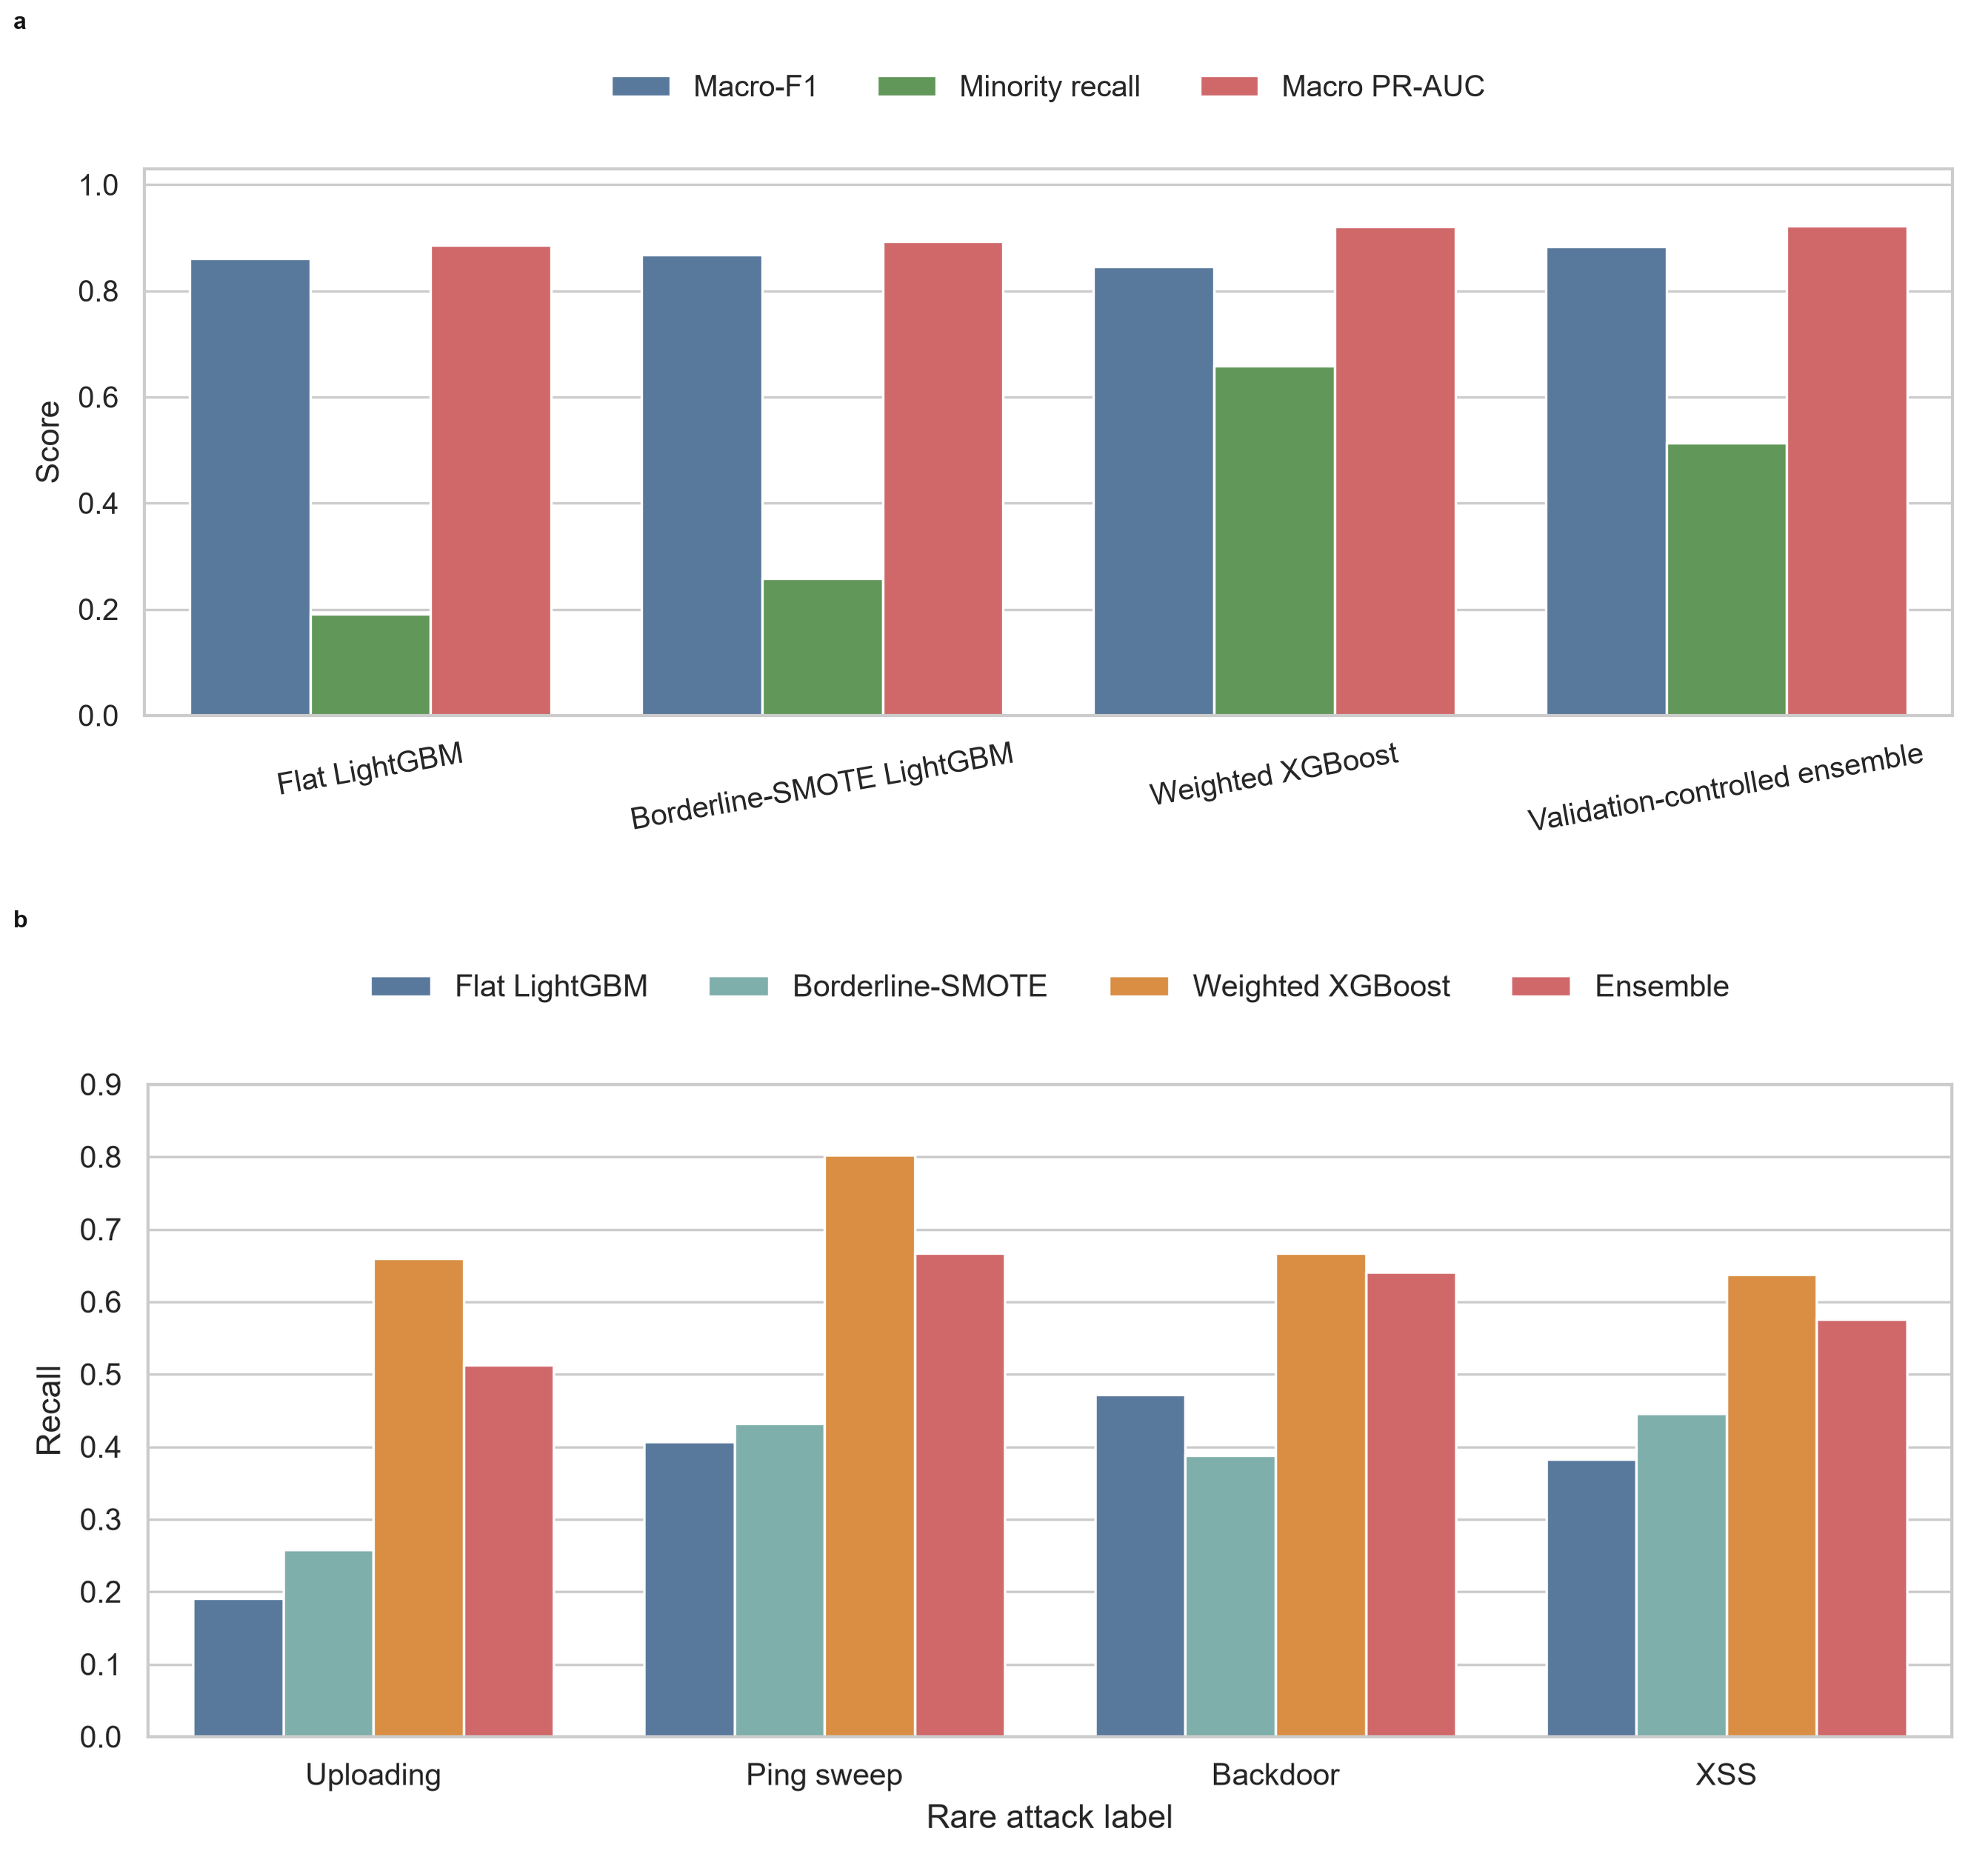
\includegraphics[width=0.98\linewidth]{figures/figure2_ciciot_performance_rare_recall.png}
\caption{\textbf{Primary CICIoT2023 public subsample performance and rare label recall.}}
\label{fig:ciciot-main}
\end{figure}

Borderline-SMOTE LightGBM preserved stronger Macro-F1 than the flat baseline. Weighted XGBoost gave the highest minority recall, but at lower Macro-F1. Probability mixing selected a middle operating point with stronger class balance than either a flat model or a recall only component.

\begin{table}[H]
\centering
\caption{\textbf{CICIoT2023 public subsample main results.} Metrics are computed on the frozen public subsample test split. The final row reports ensemble minus flat LightGBM paired row bootstrap point differences from 2,000 resamples.}
\label{tab:ciciot}
\scriptsize
\begin{tabularx}{\linewidth}{L{3.9cm} c c c c c}
\toprule
Model or comparison & Accuracy & Bal. acc. & Macro-F1 & Minority recall & Macro PR-AUC \\
\midrule
Flat LightGBM & 0.9462 & 0.8446 & 0.8612 & 0.1910 & 0.8863 \\
Borderline-SMOTE LightGBM & 0.9477 & 0.8495 & 0.8674 & 0.2584 & 0.8933 \\
Weighted XGBoost & 0.9359 & 0.8981 & 0.8453 & 0.6592 & 0.9203 \\
Validation-controlled ensemble & 0.9486 & 0.8883 & 0.8828 & 0.5131 & 0.9219 \\
Ensemble minus flat LightGBM & n/a & +0.0437 & +0.0216 & +0.3221 & n/a \\
\bottomrule
\end{tabularx}
\end{table}

Paired row bootstrap intervals supported the CICIoT2023 public subsample differences under the fixed test split. The ensemble minus flat LightGBM Macro-F1 delta was 0.0216, with a 95\% interval from 0.0186 to 0.0246. Minority recall increased by 0.3221, with a 95\% interval from 0.2635 to 0.3837. Balanced accuracy increased by 0.0437. These findings support the ensemble as the primary CICIoT2023 public subsample operating point under the fixed public subsample split.

Additional model family, SMOTEENN, class wise diagnostic and rare prior screens are reported in Supplementary Tables S12 to S17. These analyses are treated as diagnostics rather than as replacements for the frozen CICIoT2023 public subsample comparison.

\subsection*{Improvement of minority attack recognition}

To investigate whether the aggregate gain reflected rare attack recognition rather than only majority class performance, recall was examined for four low support attack labels (Figure~\ref{fig:ciciot-main}). The ensemble increased Uploading\_Attack recall from 0.1910 to 0.5131, Recon-PingSweep recall from 0.4065 to 0.6667, Backdoor\_Malware recall from 0.4719 to 0.6406 and XSS recall from 0.3827 to 0.5761. Weighted XGBoost alone gave higher recall for several rare labels. This compromise is the intended behavior: rare attacks become more visible without allowing a recall only component to dominate the final model.

Class wise diagnostics and the recall sensitive rare prior screen are reported in Supplementary Tables S13, S14 and S17. They support the same interpretation: the selected ensemble improves several rare labels, but some rare labels remain only partially recovered.

\subsection*{Cross-dataset validation}

\subsubsection*{IoTID20 repeated holdout stability}

To determine whether the imbalance aware pattern was stable beyond a single holdout, IoTID20 was evaluated with 10 repeated stratified 70/30 splits and bootstrap at the split level. Across the 10 splits, flat LightGBM achieved mean Macro-F1 0.6082 and mean minority recall 0.2691. Top ten flat LightGBM achieved mean Macro-F1 0.6113 and minority recall 0.2679. Top ten weighted LightGBM achieved mean Macro-F1 0.6222 (SD 0.0021) and minority recall 0.4820 (SD 0.0081).

The ablation separates feature selection from imbalance handling. Relative to flat LightGBM, top ten flat LightGBM improved Macro-F1 by only 0.0031 and changed minority recall by -0.0012. Top ten weighted LightGBM improved Macro-F1 by 0.0140, with a 95\% split bootstrap interval from 0.0117 to 0.0165. Minority recall increased by 0.2129, with a 95\% interval from 0.2075 to 0.2178. Exact sign flip tests gave two sided $p=0.0020$ for Macro-F1 and $p=0.0020$ for minority recall. Macro PR-AUC remained essentially unchanged: the top ten weighted LightGBM delta was 0.0001, with an interval from -0.0002 to 0.0004. The validation controlled ensemble was close, with mean Macro-F1 0.6220 and minority recall 0.4819, but it did not surpass the compact weighted LightGBM route. The stable effect is class weighting under validation control, not the specific ensemble architecture (Figure~\ref{fig:iotid}).

\begin{figure}[H]
\centering
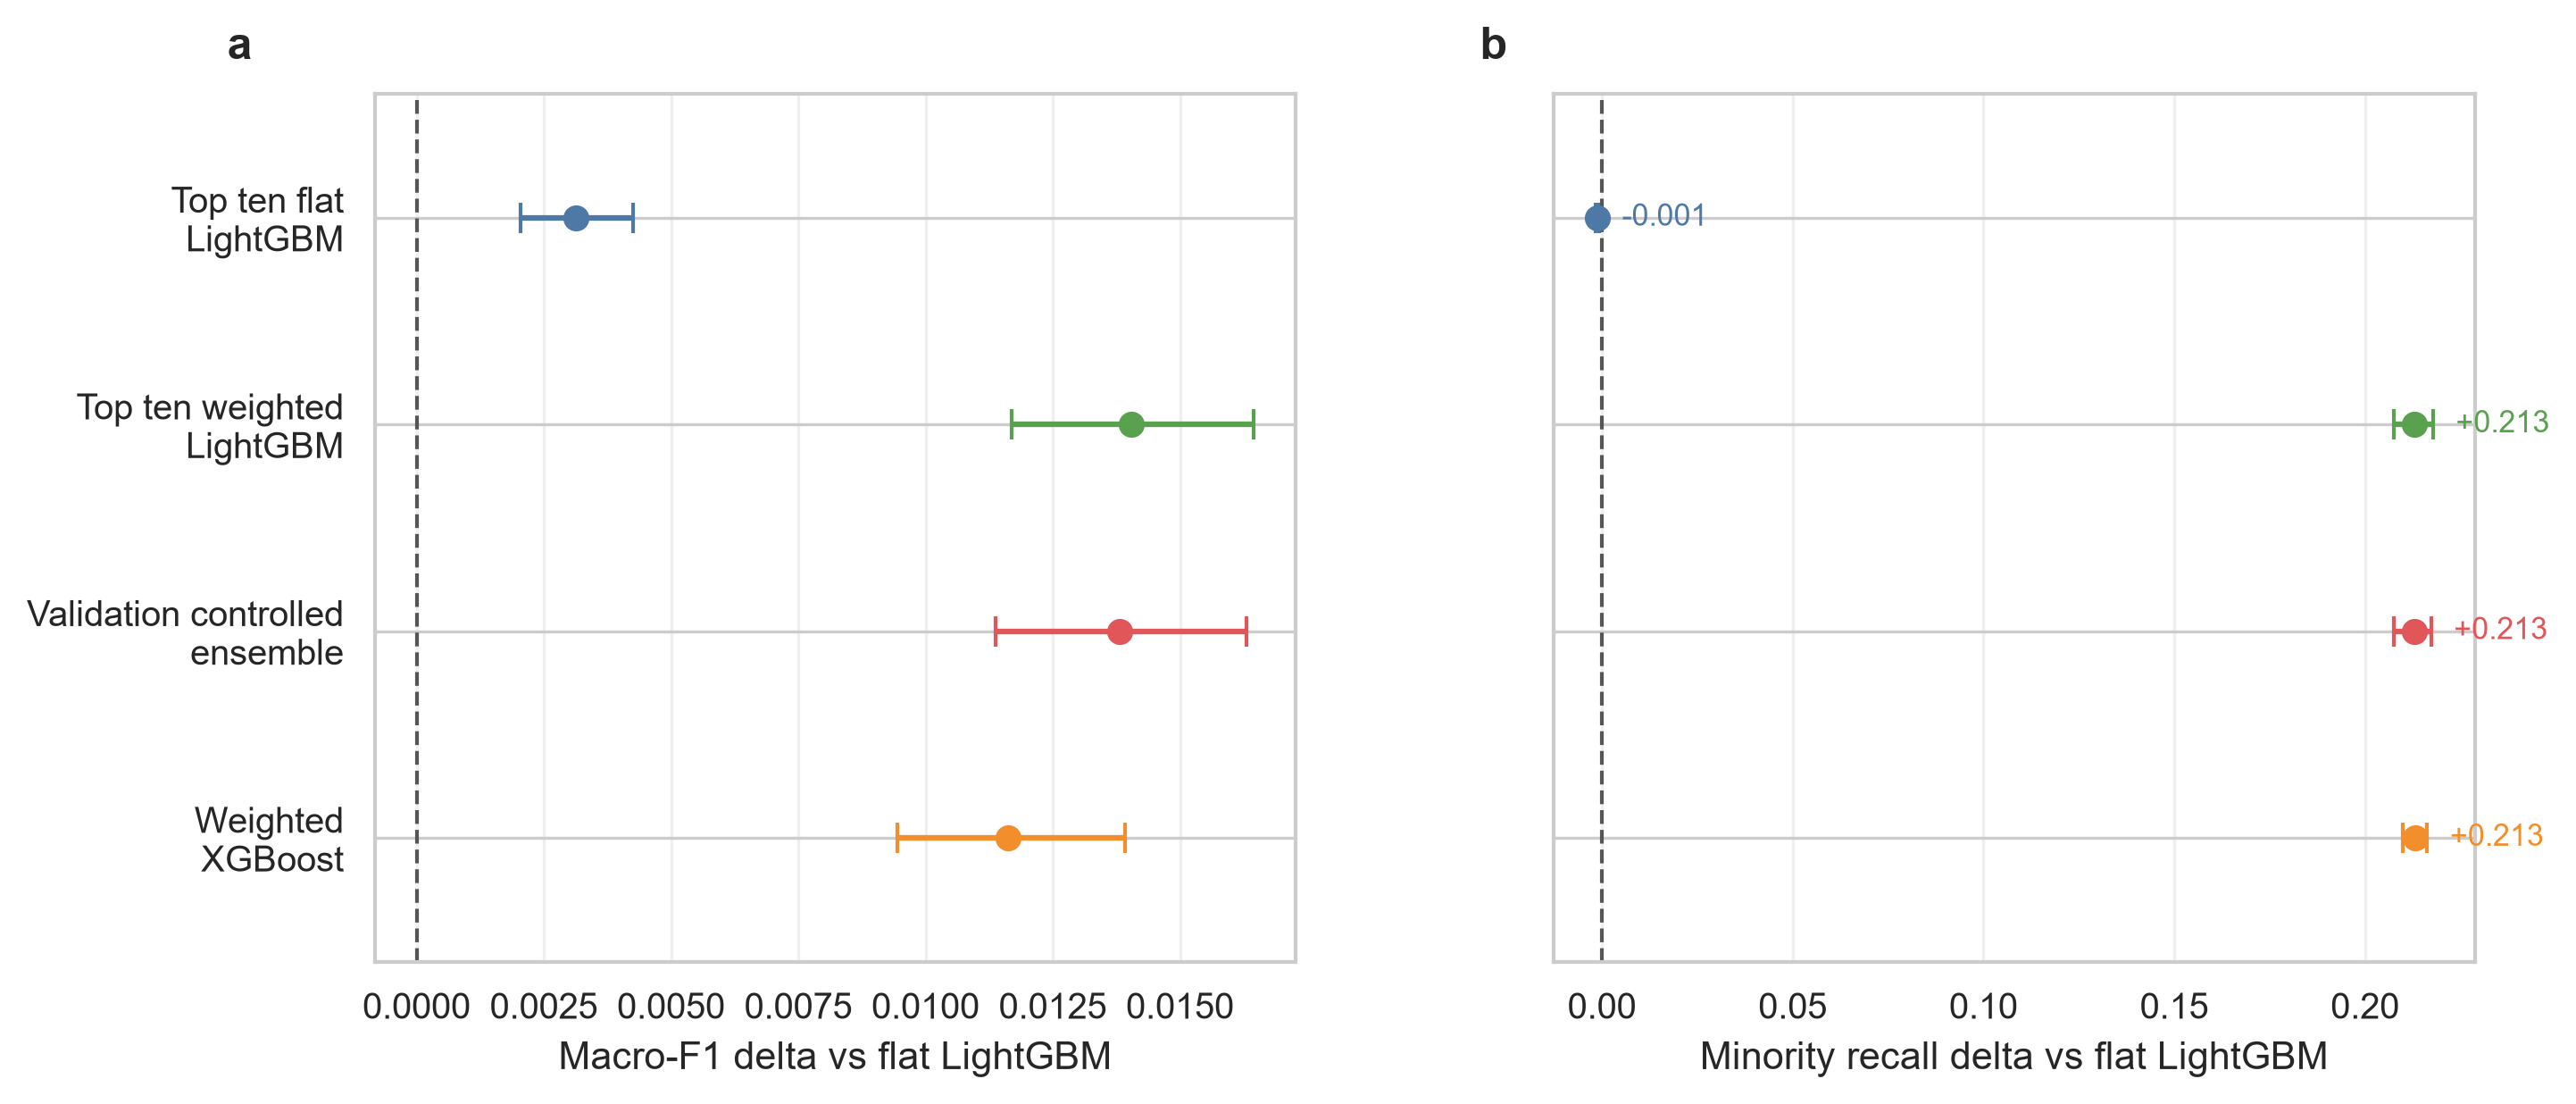
\includegraphics[width=0.98\linewidth]{figures/figure3_iotid20_repeated_split.png}
\caption{\textbf{IoTID20 repeated split validation.}}
\label{fig:iotid}
\end{figure}


\begin{table}[H]
\centering
\caption{\textbf{IoTID20 repeated holdout summary.}}
\label{tab:iotid}
\small
\begin{tabularx}{\linewidth}{L{4.4cm} c c c c}
\toprule
Model & Splits & Mean Macro-F1 & Mean minority recall & Mean PR-AUC \\
\midrule
Top ten weighted LightGBM & 10 & 0.6222 & 0.4820 & 0.6800 \\
Validation-controlled ensemble & 10 & 0.6220 & 0.4819 & 0.6799 \\
Weighted LightGBM & 10 & 0.6204 & 0.4853 & 0.6782 \\
Top ten flat LightGBM & 10 & 0.6113 & 0.2679 & 0.6817 \\
Flat LightGBM & 10 & 0.6082 & 0.2691 & 0.6798 \\
\bottomrule
\end{tabularx}
\end{table}

Supplementary Table S15 reports repeated split class wise IoTID20 diagnostics. The per class pattern is uneven, which is why the claim is written as split stable imbalance aware recall rather than dataset universal superiority.

\subsubsection*{N-BaIoT unseen-device validation}

To investigate whether performance was retained when complete devices were held out, N-BaIoT was evaluated with capped leave one device out folds. Binary and attack family settings were near saturated, with mean Macro-F1 of 0.9998 and 0.9999, respectively. Such near perfect values should be read cautiously because N-BaIoT statistics may separate benign and attack periods unusually well and because the 20,000 row per file cap may influence the apparent ceiling. Fine grained attack labels were more heterogeneous: mean Macro-F1 was 0.9435, minimum Macro-F1 was 0.7483, mean Macro-F1 for classes present in the fold was 0.9867 and the weakest present class recall across folds was 0.6917. The N-BaIoT results are best interpreted as capped sample device transfer evidence rather than a direct estimate of live deployment performance (Figure~\ref{fig:nbaiot}).

\begin{figure}[H]
\centering
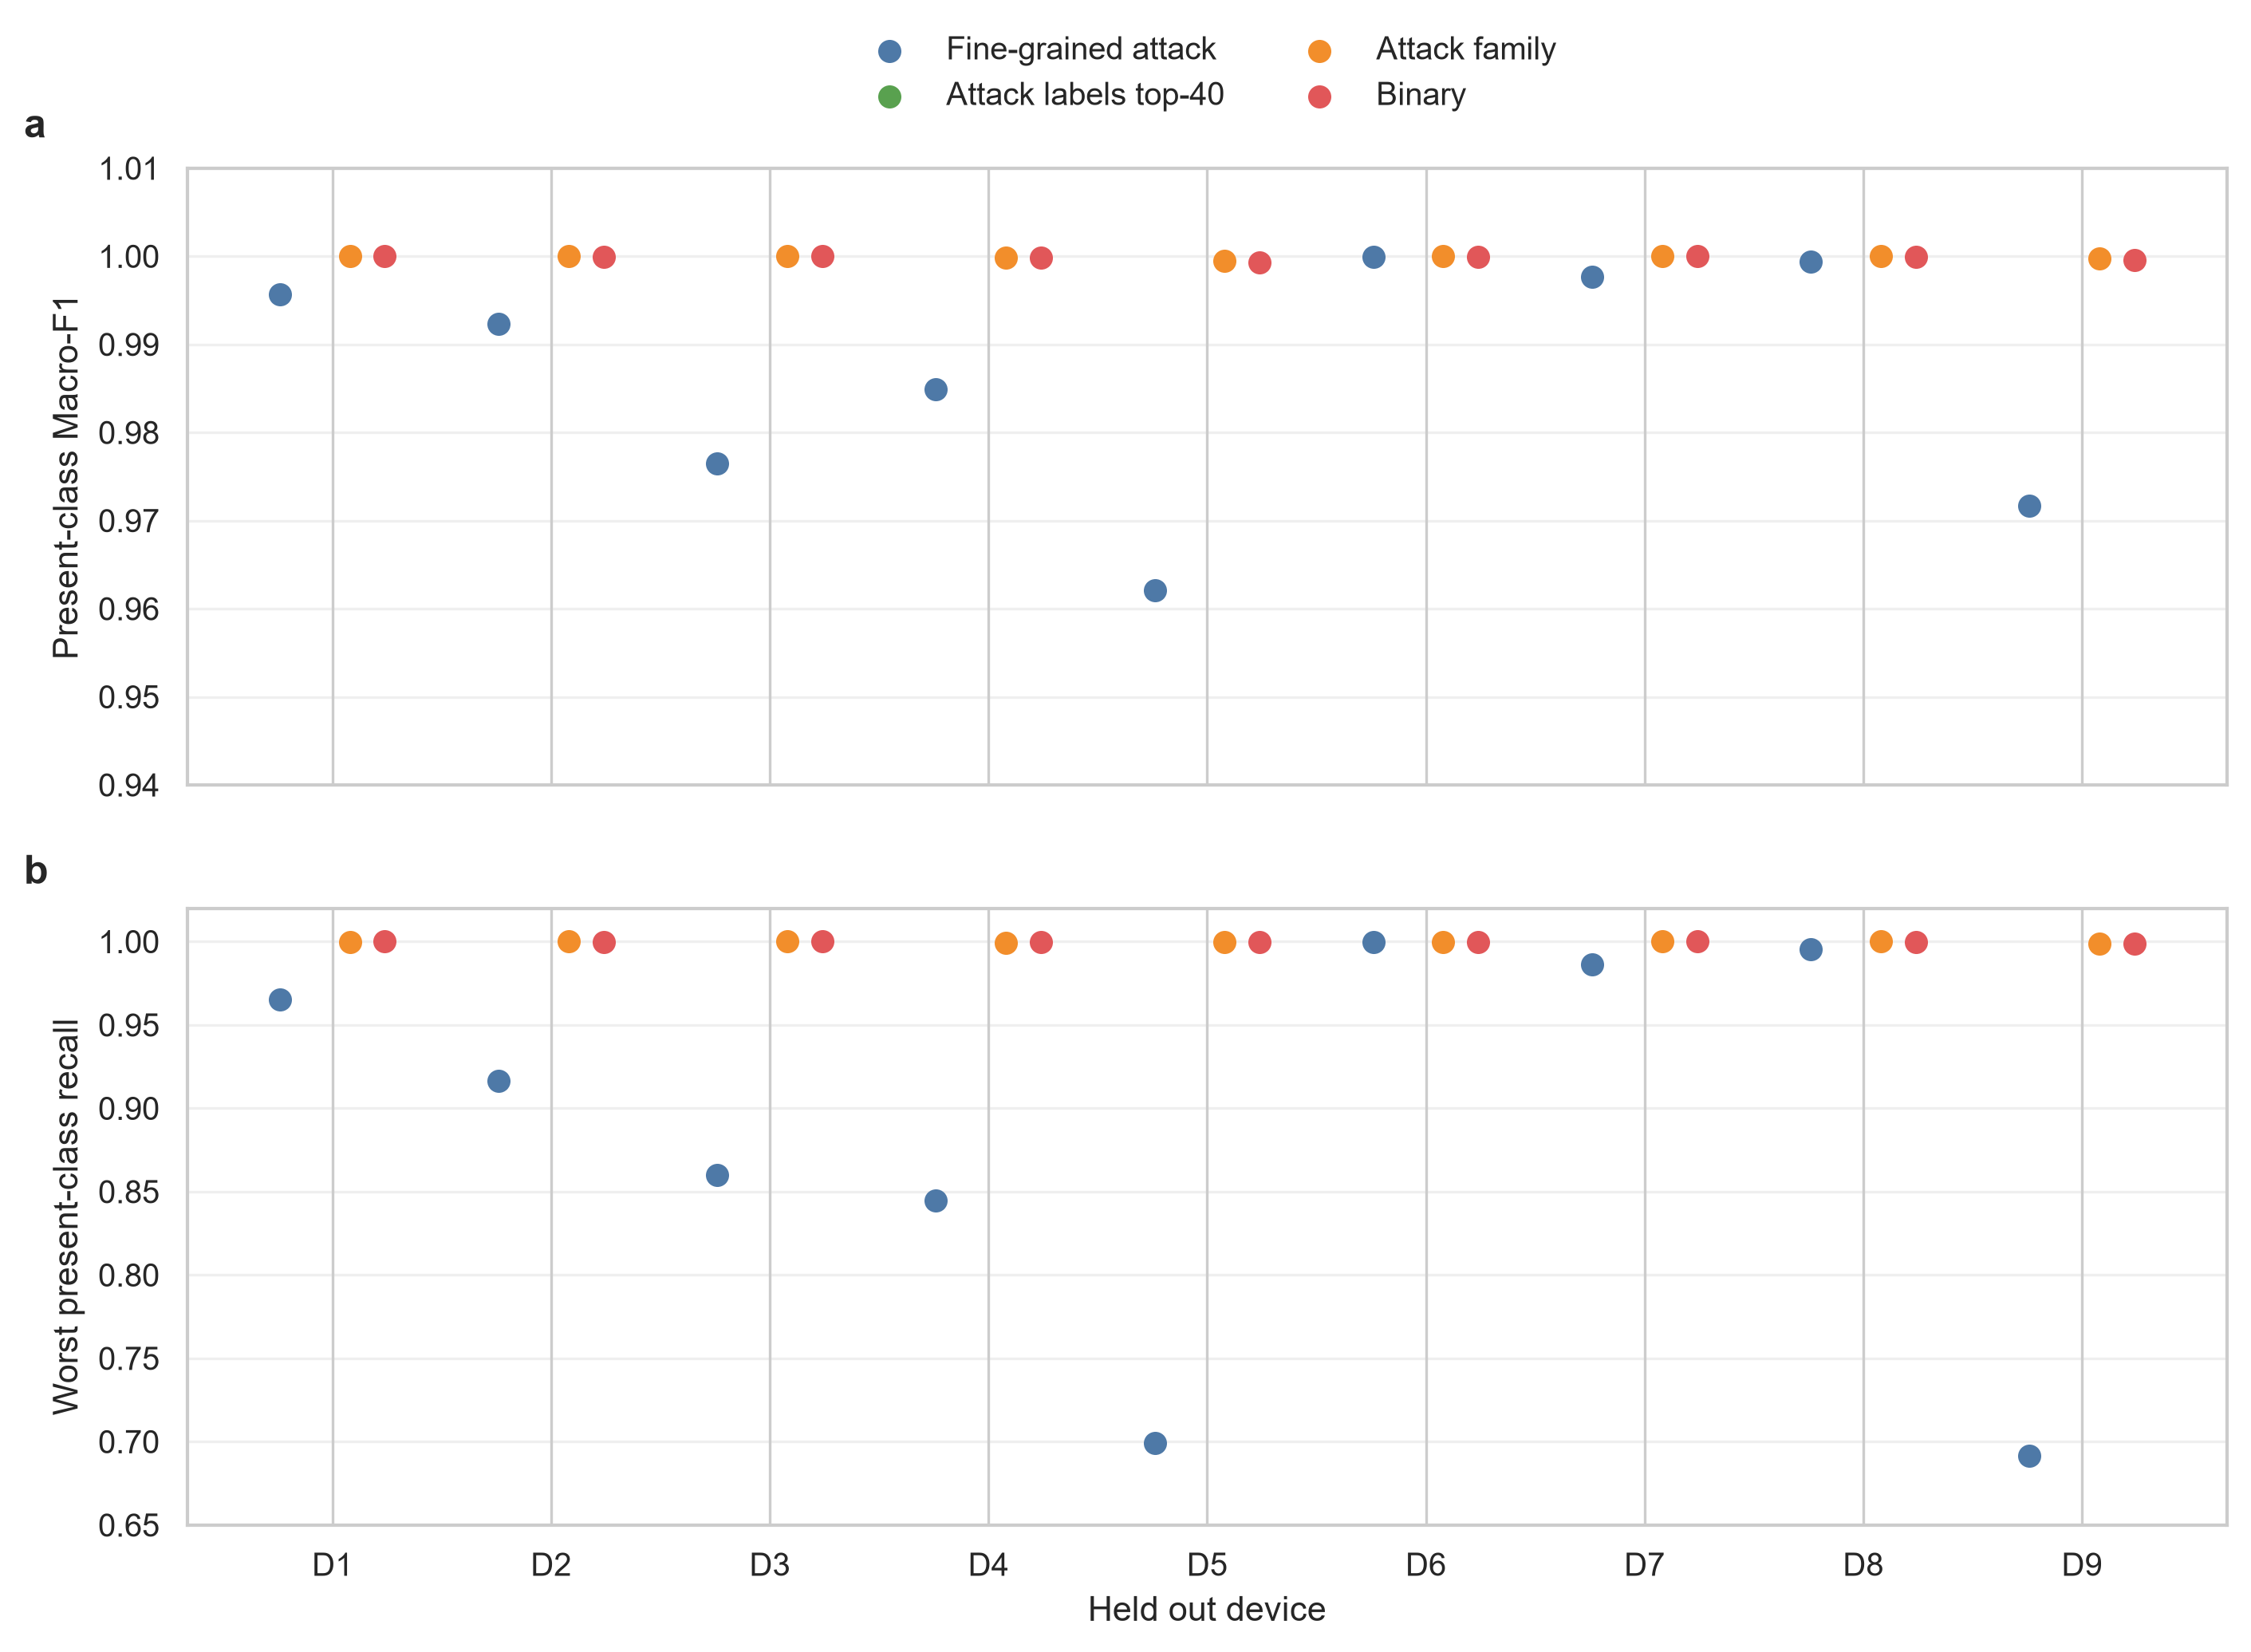
\includegraphics[width=0.98\linewidth]{figures/figure4_nbaiot_unseen_device.png}
\caption{\textbf{N-BaIoT leave one device out validation.}}
\label{fig:nbaiot}
\end{figure}


\begin{table}[H]
\centering
\caption{\textbf{N-BaIoT leave one device out summary.}}
\label{tab:nbaiot}
\small
\begin{tabularx}{\linewidth}{L{2.0cm} c c c c c}
\toprule
Task & Folds & Mean Macro-F1 & Min Macro-F1 & Mean present Macro-F1 & Min present recall \\
\midrule
attack & 9 & 0.9435 & 0.7483 & 0.9867 & 0.6917 \\
binary & 9 & 0.9998 & 0.9993 & 0.9998 & 0.9990 \\
family & 9 & 0.9999 & 0.9995 & 0.9999 & 0.9990 \\
\bottomrule
\end{tabularx}
\end{table}

Supplementary Table S16 compares the available N-BaIoT per file caps. The sensitivity table is used only to check whether the capped device transfer pattern changes materially with sample size; it does not convert N-BaIoT into live deployment evidence.

Component level SHAP analysis is reported in Supplementary Figure S1 and Supplementary Table S4. The highest ranked CICIoT2023 public subsample LightGBM features were IAT, Number, Header\_Length, Protocol Type, rst\_count, Weight, syn\_count, flow\_duration. These timing, packet size, protocol and flag count variables are plausible traffic level signals. The purpose of SHAP here is to check that the model attends to reasonable traffic features, not to identify causal features of attacks.

\section*{Discussion}

The CICIoT2023 public subsample results support validation controlled imbalance handling as a useful evaluation discipline for fine grained IoT intrusion detection. The main gain is not a claim that a new architecture dominates the field; it is that model weights, imbalance treatment and feature choices are fixed before the frozen test split is evaluated, and the result is judged with Macro-F1, minority recall, macro precision recall area and paired uncertainty rather than headline accuracy alone. Under this discipline, the validation selected ensemble improved the lowest support CICIoT2023 public subsample class while preserving a stronger overall Macro-F1 operating point than either a flat baseline or a recall only component. This is also why published high accuracy or detection rate studies are treated as benchmark context rather than direct leaderboard comparators: their datasets, label granularity, task definitions and split protocols differ from the present public subsample study.

The IoTID20 repeated holdouts limit the claim in a constructive way. They support a split stable imbalance aware recall pattern, but they do not support universal ensemble superiority. The stronger IoTID20 route was a compact top ten weighted LightGBM model, while the validation controlled ensemble remained close. This pattern indicates that class weighting under validation control is the transferable element, whereas the best architecture can shift with feature space, label set and dataset size. In practical terms, the framework provides a selection discipline for choosing among operating points, not a guarantee that probability mixing is always the best deployment model.

N-BaIoT adds a device boundary rather than a stronger claim of real world deployment. Binary and attack family tasks were nearly saturated in the capped leave one device out setting, which may reflect strong separability in engineered traffic statistics and should be read as an upper bound check. Fine grained attack labels were more heterogeneous across held out devices, making them the more informative boundary result. The study therefore supports a reproducible validation framework for imbalanced public IoT intrusion detection, while leaving concept drift, live traffic, wider multi dataset benchmarking, richer sequence or graph features and prospective deployment validation as necessary future tests.

\section*{Conclusion}

This study presents validation controlled imbalance aware learning as a reproducible framework for imbalanced IoT intrusion detection.

The scientific finding is that rare class recall can be improved when imbalance treatment, feature choice and ensemble weighting are fixed by internal validation rather than by the final test split.

The implication is broader than one dataset: imbalanced security classifiers should be judged by validation discipline, rare-label metrics and explicit boundary tests, not by headline accuracy alone.

\section*{Data availability}

The datasets used in this study are publicly available. No new primary data were generated. CICIoT2023 public subsample: \url{https://huggingface.co/datasets/lacg030175/CIC-IoT-2023-neto-subsample}. Original CICIoT2023 project page: \url{https://www.unb.ca/cic/datasets/iotdataset-2023.html}. IoTID20 preprocessed file: \url{https://huggingface.co/datasets/KathiS/IoTID20_Preprocessed_File}. N-BaIoT UCI archive: \url{https://archive.ics.uci.edu/dataset/442/detection+of+iot+botnet+attacks+n+baiot}.

\section*{Code availability}

The reproducibility package is publicly available at GitHub: \url{https://github.com/williamjay1/validation-controlled-iot-ids}. The archived Zenodo release is available at \url{https://doi.org/10.5281/zenodo.21272745}. The archive contains executable scripts, pinned environment requirements, generated result CSV files, figure generation code, manuscript source files and checksum records for the submitted outputs.


\begin{thebibliography}{99}

\bibitem{alfuqaha2015iot}
Al-Fuqaha, A., Guizani, M., Mohammadi, M., Aledhari, M. \& Ayyash, M. Internet of Things: A survey on enabling technologies, protocols, and applications. \emph{IEEE Commun. Surv. Tutor.} \textbf{17}, 2347--2376 (2015). doi: \url{https://doi.org/10.1109/COMST.2015.2444095}.

\bibitem{roman2013iotsecurity}
Roman, R., Zhou, J. \& Lopez, J. On the features and challenges of security and privacy in distributed internet of things. \emph{Comput. Netw.} \textbf{57}, 2266--2279 (2013). doi: \url{https://doi.org/10.1016/j.comnet.2012.12.018}.

\bibitem{sicari2015iottrust}
Sicari, S., Rizzardi, A., Grieco, L. A. \& Coen-Porisini, A. Security, privacy and trust in Internet of Things: The road ahead. \emph{Comput. Netw.} \textbf{76}, 146--164 (2015). doi: \url{https://doi.org/10.1016/j.comnet.2014.11.008}.

\bibitem{neto2023ciciot}
Neto, E. C. P. et al. CICIoT2023: A real-time dataset and benchmark for large-scale attacks in IoT environment. \emph{Sensors} \textbf{23}, 5941 (2023). doi: \url{https://doi.org/10.3390/s23135941}.

\bibitem{ullah2020iotid20}
Ullah, I. \& Mahmoud, Q. H. A scheme for generating a dataset for anomalous activity detection in IoT networks. In \emph{Advances in Artificial Intelligence}, Lecture Notes in Computer Science \textbf{12109}, 508--520 (Springer, 2020). doi: \url{https://doi.org/10.1007/978-3-030-47358-7_52}.

\bibitem{meidan2018nbaiot}
Meidan, Y. et al. N-BaIoT: Network based detection of IoT botnet attacks using deep autoencoders. \emph{IEEE Pervasive Comput.} \textbf{17}, 12--22 (2018). doi: \url{https://doi.org/10.1109/MPRV.2018.03367731}.

\bibitem{moustafa2015unsw}
Moustafa, N. \& Slay, J. UNSW-NB15: a comprehensive data set for network intrusion detection systems. In \emph{2015 Military Communications and Information Systems Conference}, 1--6 (2015). doi: \url{https://doi.org/10.1109/MilCIS.2015.7348942}.

\bibitem{sharafaldin2018cicids}
Sharafaldin, I., Lashkari, A. H. \& Ghorbani, A. A. Toward generating a new intrusion detection dataset and intrusion traffic characterization. In \emph{Proceedings of the 4th International Conference on Information Systems Security and Privacy}, 108--116 (2018). doi: \url{https://doi.org/10.5220/0006639801080116}.

\bibitem{koroniotis2019botiot}
Koroniotis, N., Moustafa, N., Sitnikova, E. \& Turnbull, B. Towards the development of realistic botnet dataset in the Internet of Things for network forensic analytics: Bot-IoT dataset. \emph{Future Gener. Comput. Syst.} \textbf{100}, 779--796 (2019). doi: \url{https://doi.org/10.1016/j.future.2019.05.041}.

\bibitem{ferrag2022edgeiiot}
Ferrag, M. A., Friha, O., Hamouda, D., Maglaras, L. \& Janicke, H. Edge-IIoTset: A new comprehensive realistic cyber security dataset of IoT and IIoT applications for centralized and federated learning. \emph{IEEE Access} \textbf{10}, 40281--40306 (2022). doi: \url{https://doi.org/10.1109/ACCESS.2022.3165809}.

\bibitem{he2009imbalanced}
He, H. \& Garcia, E. A. Learning from imbalanced data. \emph{IEEE Trans. Knowl. Data Eng.} \textbf{21}, 1263--1284 (2009). doi: \url{https://doi.org/10.1109/TKDE.2008.239}.

\bibitem{branco2016imbalanced}
Branco, P., Torgo, L. \& Ribeiro, R. P. A survey of predictive modeling on imbalanced domains. \emph{ACM Comput. Surv.} \textbf{49}, 1--50 (2016). doi: \url{https://doi.org/10.1145/2907070}.

\bibitem{krawczyk2016imbalanced}
Krawczyk, B. Learning from imbalanced data: open challenges and future directions. \emph{Prog. Artif. Intell.} \textbf{5}, 221--232 (2016). doi: \url{https://doi.org/10.1007/s13748-016-0094-0}.

\bibitem{chen2016xgboost}
Chen, T. \& Guestrin, C. XGBoost: A scalable tree boosting system. In \emph{Proceedings of the 22nd ACM SIGKDD International Conference on Knowledge Discovery and Data Mining}, 785--794 (2016). doi: \url{https://doi.org/10.1145/2939672.2939785}.

\bibitem{chawla2002smote}
Chawla, N. V., Bowyer, K. W., Hall, L. O. \& Kegelmeyer, W. P. SMOTE: Synthetic minority over sampling technique. \emph{J. Artif. Intell. Res.} \textbf{16}, 321--357 (2002). doi: \url{https://doi.org/10.1613/jair.953}.

\bibitem{han2005borderline}
Han, H., Wang, W.-Y. \& Mao, B.-H. Borderline-SMOTE: A new over sampling method in imbalanced data sets learning. In \emph{Advances in Intelligent Computing}, Lecture Notes in Computer Science \textbf{3644}, 878--887 (Springer, 2005). doi: \url{https://doi.org/10.1007/11538059_91}.

\bibitem{galar2012ensembles}
Galar, M., Fernandez, A., Barrenechea, E., Bustince, H. \& Herrera, F. A review on ensembles for the class imbalance problem: Bagging, boosting, and hybrid based approaches. \emph{IEEE Trans. Syst. Man Cybern. C} \textbf{42}, 463--484 (2012). doi: \url{https://doi.org/10.1109/TSMCC.2011.2161285}.

\bibitem{alsubaei2025smart}
Alsubaei, F. S. Smart deep learning model for enhanced IoT intrusion detection. \emph{Sci. Rep.} \textbf{15}, 20577 (2025). doi: \url{https://doi.org/10.1038/s41598-025-06363-5}.

\bibitem{yu2025attack}
Yu, Y., Fu, Y., Liu, T., Wang, K. \& An, Y. An attack detection method based on deep learning for internet of things. \emph{Sci. Rep.} \textbf{15}, 28812 (2025). doi: \url{https://doi.org/10.1038/s41598-025-14808-0}.

\bibitem{amine2025improved}
Amine, M. S., Nada, F. A. \& Hosny, K. M. Improved model for intrusion detection in the Internet of Things. \emph{Sci. Rep.} \textbf{15}, 21547 (2025). doi: \url{https://doi.org/10.1038/s41598-025-92852-6}.

\bibitem{ma2025llm}
Ma, H., Zhang, W., Zhang, D. \& Chen, B. An IoT intrusion detection framework based on feature selection and large language models fine-tuning. \emph{Sci. Rep.} \textbf{15}, 21158 (2025). doi: \url{https://doi.org/10.1038/s41598-025-08905-3}.

\bibitem{sarwar2025securing}
Sarwar, N., Alharthi, R. S., Aljohani, M. \& Elhosseini, M. A. Securing IoT networks: a machine learning approach for detecting unusual traffic patterns. \emph{Sci. Rep.} \textbf{15}, 3397 (2025). doi: \url{https://doi.org/10.1038/s41598-025-33447-z}.

\bibitem{singh2025attentional}
Singh, R., Singh Gill, N. \& Gulia, P. Attentional LSTM-ensemble architecture for intrusion detection in smart grids. \emph{Sci. Rep.} \textbf{15}, 41977 (2025). doi: \url{https://doi.org/10.1038/s41598-025-25992-4}.

\bibitem{abushareha2026review}
Abu-Shareha, A. A. et al. Supervised machine learning intrusion detection review and multi criteria evaluation. \emph{Sci. Rep.} \textbf{16}, 14525 (2026). doi: \url{https://doi.org/10.1038/s41598-026-44773-1}.

\bibitem{davis2006pr}
Davis, J. \& Goadrich, M. The relationship between Precision-Recall and ROC curves. In \emph{Proceedings of the 23rd International Conference on Machine Learning}, 233--240 (2006). doi: \url{https://doi.org/10.1145/1143844.1143874}.

\bibitem{saito2015pr}
Saito, T. \& Rehmsmeier, M. The Precision-Recall plot is more informative than the ROC plot when evaluating binary classifiers on imbalanced datasets. \emph{PLoS ONE} \textbf{10}, e0118432 (2015). doi: \url{https://doi.org/10.1371/journal.pone.0118432}.

\bibitem{efron1979bootstrap}
Efron, B. Bootstrap methods: another look at the jackknife. \emph{Ann. Stat.} \textbf{7}, 1--26 (1979). doi: \url{https://doi.org/10.1214/aos/1176344552}.

\bibitem{efron1987bca}
Efron, B. Better bootstrap confidence intervals. \emph{J. Am. Stat. Assoc.} \textbf{82}, 171--185 (1987). doi: \url{https://doi.org/10.1080/01621459.1987.10478410}.

\bibitem{dietterich1998tests}
Dietterich, T. G. Approximate statistical tests for comparing supervised classification learning algorithms. \emph{Neural Comput.} \textbf{10}, 1895--1923 (1998). doi: \url{https://doi.org/10.1162/089976698300017197}.

\bibitem{ernst2004permutation}
Ernst, M. D. Permutation methods: a basis for exact inference. \emph{Stat. Sci.} \textbf{19}, 676--685 (2004). doi: \url{https://doi.org/10.1214/088342304000000396}.

\bibitem{lundberg2020shap}
Lundberg, S. M. et al. From local explanations to global understanding with explainable AI for trees. \emph{Nat. Mach. Intell.} \textbf{2}, 56--67 (2020). doi: \url{https://doi.org/10.1038/s42256-019-0138-9}.

\end{thebibliography}


\section*{Acknowledgements}

This research was funded by the National Social Science Fund of China (General Program), grant 25BGJ089.

\section*{Author contributions statement}

J.Z. and S.W. conceived the study. J.Z. curated the data, implemented the experiments, analysed the results and prepared the first draft. S.W. supervised the study, contributed to methodology and reviewed and edited the manuscript. Both authors approved the final manuscript.

\section*{Additional information}

\textbf{Competing interests} The authors declare no competing interests. \textbf{Ethics statement} This study used publicly available network intrusion datasets and did not involve human participants, human tissue or animal subjects. \textbf{Generative AI and tool-use disclosure} AI-assisted coding and drafting tools were used as described in Methods; the authors remain responsible for the manuscript, code and numerical claims.

\end{document}
